\documentclass{standalone}
\usepackage{tikz}
\usetikzlibrary{positioning,fit,arrows}
\begin{document}
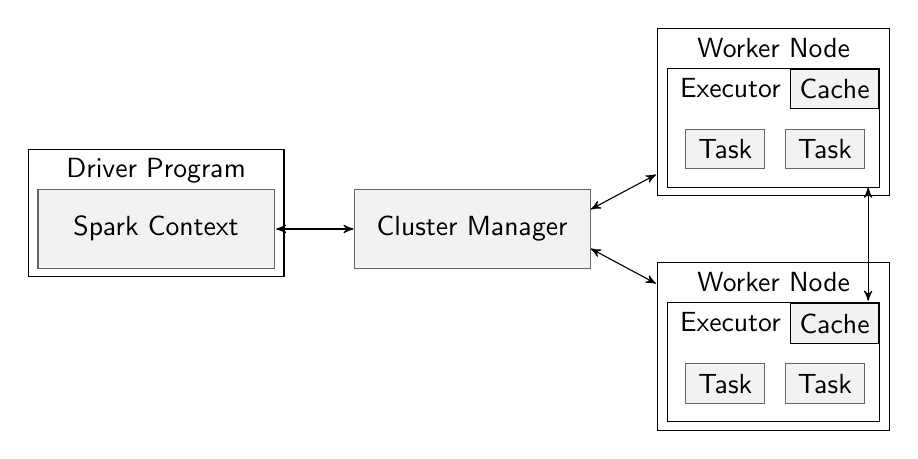
\begin{tikzpicture}[
        node/.style={
                rectangle,
                draw=black!60,
                fill=black!5,
                text centered,
                minimum width=30mm,
                minimum height=10mm,
            },
        task/.style={
                rectangle,
                draw=black!60,
                fill=black!5,
                text centered,
                minimum width=10mm,
                minimum height=5mm,
            },
        cache/.style={
                rectangle,
                draw=black,
                fill=black!5,
                text centered,
                minimum width=10mm,
                minimum height=5mm,
            },
        >= stealth',
        shorten >= 0.5pt
    ]
    \node[node,font=\sffamily] (cluster) {Cluster Manager};
    \node[node,font=\sffamily] (sparkContext) [left=1cm of cluster] {Spark Context};
    \node[task,font=\sffamily] (task11) [above right=0.25cm and 1.2cm of cluster] {Task};
    \node[task,font=\sffamily] (task12) [right=0.25cm of task11] {Task};
    \node[task,font=\sffamily] (task21) [below right=1.2cm and 1.2cm of cluster] {Task};
    \node[task,font=\sffamily] (task22) [right=0.25cm of task21] {Task};
    \node[cache,font=\sffamily] (cache1) [above right=0.25cm and -0.95cm of task12] {Cache};
    \node[cache,font=\sffamily] (cache2) [above right=0.25cm and -0.95cm of task22] {Cache};

    \node[
        fit={(sparkContext)},
        draw,
        inner ysep=0.3cm,
        yshift=0.2cm,
        label={[yshift=-0.55cm, font=\sffamily]Driver Program}
    ] (driver) {};
    \node[
        fit={(task11)(task12)(cache1)},
        draw,
        xshift=-0.11cm,
        yshift=-0.11cm,
        label={[xshift=-0.55cm,yshift=-0.5cm,font=\sffamily]Executor}
    ](tasks1) {};
    \node[
        fit={(task21)(task22)(cache2)},
        draw,
        xshift=-0.11cm,
        yshift=-0.11cm,
        label={[xshift=-0.55cm,yshift=-0.5cm,font=\sffamily]Executor}
    ] (tasks2) {};
    \node[
        fit={(tasks1)},
        draw,
        inner ysep=0.3cm,
        yshift=0.2cm,
        label={[yshift=-0.5cm,font=\sffamily]Worker Node}
    ] (worker1) {};
    \node[
        fit={(tasks2)},
        draw,
        inner ysep=0.3cm,
        yshift=0.2cm,
        label={[yshift=-0.5cm,font=\sffamily]Worker Node}
    ] (worker2) {};

    \path[<->] (cluster) edge node {} (sparkContext);
    \path[<->] ([yshift=0.25cm]cluster.east) edge node {} (worker1);
    \path[<->] ([yshift=-0.25cm]cluster.east) edge node {} (worker2);
    \path[<->] ([xshift=1.2cm]tasks1.south) edge node[right] {} ([xshift=1.2cm]tasks2.north);
\end{tikzpicture}
\end{document}